\documentclass[12pt]{article}
\usepackage[margin=1in]{geometry}
\usepackage{hyperref}
\usepackage{multicol}
\usepackage{upgreek}
\usepackage{graphicx}
\usepackage[section]{placeins} % Keeps images within their section. 
\DeclareGraphicsExtensions{.pdf,.png,.jpg}

%perhaps comment this out later. 
\newcommand{\Sum}[3]{\sum_{#1}^{#2} #3}

\pdfinfo{%
  /Title    (Project1)
  /Author   (Clinton McKay)
  /Creator  (Clinton McKay)
  /Producer (Clinton McKay)
  /Subject  (CSCI 444 -- Data Visualization) 
  /Keywords (CSCI444)
}

\title{Final Project: UN Homicides\\ {\Large Good \& Bad Visuals}}
\date{\today}
\author{Clinton McKay}

\begin{document}

\maketitle

\section{Other Visuals}

\subsection{Good Supporting Visual} 
I felt that this was a good visual. The primary reason is that author chose a set of good colors. The use of red and blue catch the eye as either good or bad trends. For example it is evident that the USA has too many inmates (more than Russia). If a country does not have any associated data then the pale-yellow fill makes it noticeable and keeps it separate from the other colors.

\begin{figure}[!ht]
    \centering
    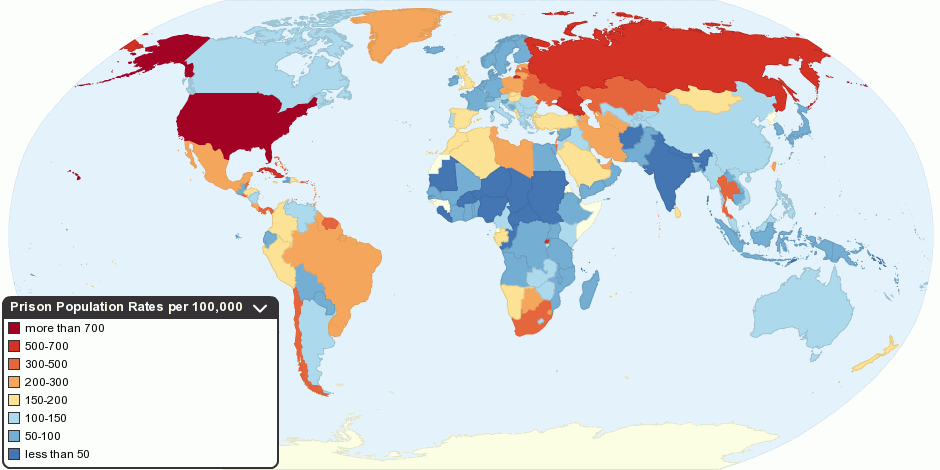
\includegraphics[width=6in, keepaspectratio]{good-visual.png}
    \caption{Stress forces on a hook.}
    \label{fig:example_good}
\end{figure}

\subsection{Bad Supporting Visual for a Hypothesis}
This graph is overkill. The author displays 2D data in a 3D plot which violates one of Tufte's fundamental rules. Also, by making the graph 3D it has become difficult to compare the rates amongst the different countries. 

\begin{figure}[!ht]
    \centering
    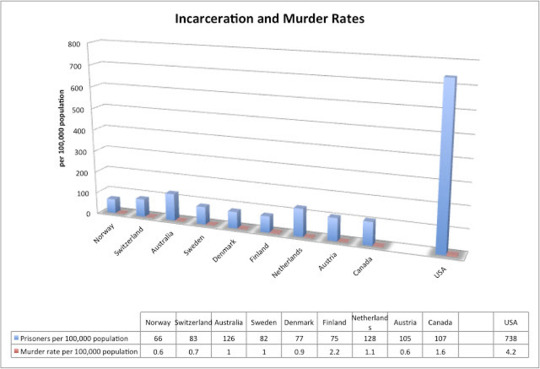
\includegraphics[width=6in, keepaspectratio]{bad-visual.jpg}
    \caption{That 3D effect sure helps clarify the data!}
    \label{fig:example_bad}
\end{figure}


\end{document}
